\documentclass[12 pt]{article}

\usepackage[utf8]{inputenc}
\usepackage[ngerman]{babel}

\usepackage{hyperref}
\usepackage[nameinlink]{cleveref}
\crefname{figure}{Abb.}{Abb.}

\usepackage{pflichtenheft}
\usepackage{svg}
\begin{document}

%TODO
\subsection{Produktübersicht}

Der \textbf{FR}aunhofer\textbf{O}penSource\textbf{S}ensor\textbf{T}ings-Server des Fraunhofer IOSB ist eine Open-Source-Implementierung des SensorThings-Standards des OGC und unter https://github.com/FraunhoferIOSB/FROST-Server downloadbar. Der FROST-Server dient der Speicherung und Verwaltung von Sensordaten.\\
Unsere Software stellt zu diesem Server eine einfache und dennoch stark konfigurierbare Weboberfläche bereit, die es ermöglicht Sensordaten aus einer Tabelle einzulesen, zu konvertieren und auf einen FROST-Server zu übertragen. Die Software läuft in einer Java JRE und das zugehörige Webinterface soll über einen herkömmlichen PC, einen Laptop oder ein Tablet erreichbar sein.\\


\subsection{Musskriterien}
\begin{enumerate}
	\item Import von Tabellen \\
	Die Daten sollen aus Tabellen im CSV-/XLSX-Format importiert werden
	\item Konvertierung des Formats der Sensordaten \\
	Die Daten sollen aus der Tabelle in ein einheitliches Format nach Vorgabe der SensorThings API konvertiert werden. Damit entsprechen sie dem Format der Daten auf einem FROST-Server.
	\item Erstellen, abspeichern, laden von Konfigurationen \\
	Die Konfiguration der Software (ausgew. Thing, Server, Format) soll gespeichert und dem Nutzer via Download einer CFG-Datei bereitgestellt werden. Eine Konfiguration soll später auch wieder geladen werden können.
	\item Datentyptransformationen \\
	Ein Wert als bspw. String soll nicht als String auf den FROST-Server übertragen werden sollen, sondern von der Software vorher in einen passenden Datentyp (bspw. Integer) umgewandelt werden
	\item Verarbeiten von Sonderwerten (Magic Numbers) \\
	Diese Werte sollen von der Software ignoriert und gegen einen NULL-Wert (o.ä.) ausgetauscht werden, bevor sie auf den FROST-Server übertragen werden.
	\item Import von Fremdquellen wie anderen Webseiten \\
	Es soll möglich sein als Quelldatei auch einen entfernten Speicherort, zum Beispiel einen Weblink  anzugeben.
	\item Weitergabe von Fehlermeldungen an den Nutzer, falls Import schief läuft \\
	Bei Fehlern in der Verarbeitung oder in der Übertragung soll der Nutzer eine Rückmeldung kriegen
	\item Logging \\
	Sämtliche Eingaben und Interaktionen des Nutzers mit der Software sollen in einer Log-Datei gespeichert werden
\end{enumerate}

\subsection{Wunschkriterien}
\begin{enumerate}
	\item Sprachauswahl: Deutsch/Englisch
	\item Bereitstellen einer Vorauswahl \\
	Dem Benutzer wird eine vorgefertigte Standard-Konfiguration bereitgestellt.
	\item Überprüfung auf Duplikate \\
	Beim Upload der Daten auf den FROST-Server werden diese mit den bestehenden Daten abgeglichen und Duplikate werden nicht erneut gespeichert.
	\item Korrektur von falschen Daten \\
	Der Benutzer hat die Möglichkeit Fehler in den Daten direkt zu korrigieren.
	\item Rückgabe nicht bearbeiteter Datensätze in neuer CSV-Datei \\
	Bei (teilweise) fehlgeschlagener Übertragung zum FROST-Server werden die nicht übertragenen Daten in einer CSV-Datei an den Benutzer zurückgegeben.
	\item Docker-Container \\
	Zur einfachen Installation steht das Programm als Docker-Container zur Verfügung
	\item Auswahl komplexer Transformationen/Aggregationen (Zusammenlegen von Daten) wie Summe, Minimum/Maximum, Durchschnitt etc.\\ 
	Zusätzliche Informationen über ausgewählte Daten werden dem Benutzer in einem Webinterface bereitgestellt.
	\item Automatisierte Daten-Aktualisierung \\
	Bei Import von Daten von einer entfernten Adresse wird eine automatische, regelmäßige Übertragung angeboten.
	\item Import kompletter Datensätze von anderem FROST-Server \\
	Der Benutzer hat zusätzlich die Möglichkeit, Daten von einem anderen FROST-Server zu kopieren
	\item Automatisierte Erkennung des Formats \\
	Aus der CSV-/XLSX-Datei werden Formate automatisch erkannt.
	
	
\end{enumerate}

\subsection{Abgrenzungskriterien}
\begin{enumerate}
	\item Keine Verwaltung von Sensor-Daten auf dem FROST-Server \\
	Die Software soll keine schon auf dem FROST-Server liegenden Daten verwalten, ändern oder löschen
\end{enumerate}


\subsection{Anwendungsbereiche}
Überall wo Daten im CSV-Format verarbeitet werden müssen: \\
Die Software soll überall dort eingesetzt werden, wo Daten aus Tabellen importiert, konvertiert und auf den FROST-Server übertragen werden sollen. \\
Hierzu zählt:
\begin{itemize}
	\item Der Import von neuen Sensordaten, welche in CSV-/XSLX-Tabellen-Form vorliegen
	\item Die Integration von bestehenden (archivierten) Sensordaten, welche in CSV-/XLSX-Tabellen-Form vorliegen
\end{itemize}

%TODO Die zwei Zielgruppen genauer darstellen/abgrenzen
\subsection{Zielgruppen}
Die Software ist auf zwei Zielgruppen ausgelegt.\\
Zum einen gibt es die Personen, welche einfach Sensordaten auf einen Frostserver laden möchten,  ohne die Konfigurationen zu ändern. \\Der Fokus liegt bei dieser Gruppe auf der einfachen Bedienung der Software.\\
Zum Anderen gibt es die Nutzergruppe die ihre eigenen Konfigurationen erstellt. Für diese Nutzergruppe ist es wichtig, dass sie komplexe Einstellungsmöglichkeiten in den Konfigurationen nutzen kann.

\subsection{Betriebsbedingungen}
Unterschieden wird zwischen Endgerät und Server. \\
Das Ziel-Endgerät ist ein Computer, wobei jedes Gerät mit einer Internetanbindung zum Programmserver, einem Webbrowser und aktiviertem JavaScript ausreichend ist.\\
\ \\
Der Programmserver benötigt eine Anbindung an den FROST-Server und das Endgerät sowie eine Java JRE.
\begin{itemize}
	\item Browser
	\item JavaScript
	\item Verbindung zum Programmserver
\end{itemize}
\begin{itemize}
	\item Verbindung zum FROST-Server
	\item Java JRE
	\item Anbindung an Endgerät (zB Internet)
\end{itemize}

\subsection{Produktumgebung}
Die Software soll plattformunabhängig auf einem Server mit minimaler Rechen- und Speicherkapazität laufen. Des weiteren soll das Programm head-less ununterbrochen funktionieren.\\ Der Server stellt die Java JRE zur Verfügung, auf dem die Software läuft. Die Software benötigt nur noch eine Verbindung zu einer FROST-Server-Instanz, welche ihm vom Nutzer in der Konfiguration gegeben wird.

\begin{itemize}
	\item head-less Server
	\item Linux/Windows Server
	\item Java JRE
	\item SensorThings API
\end{itemize}

\subsection{Seitenentwürfe}


\begin{figure}[ht]
\centering
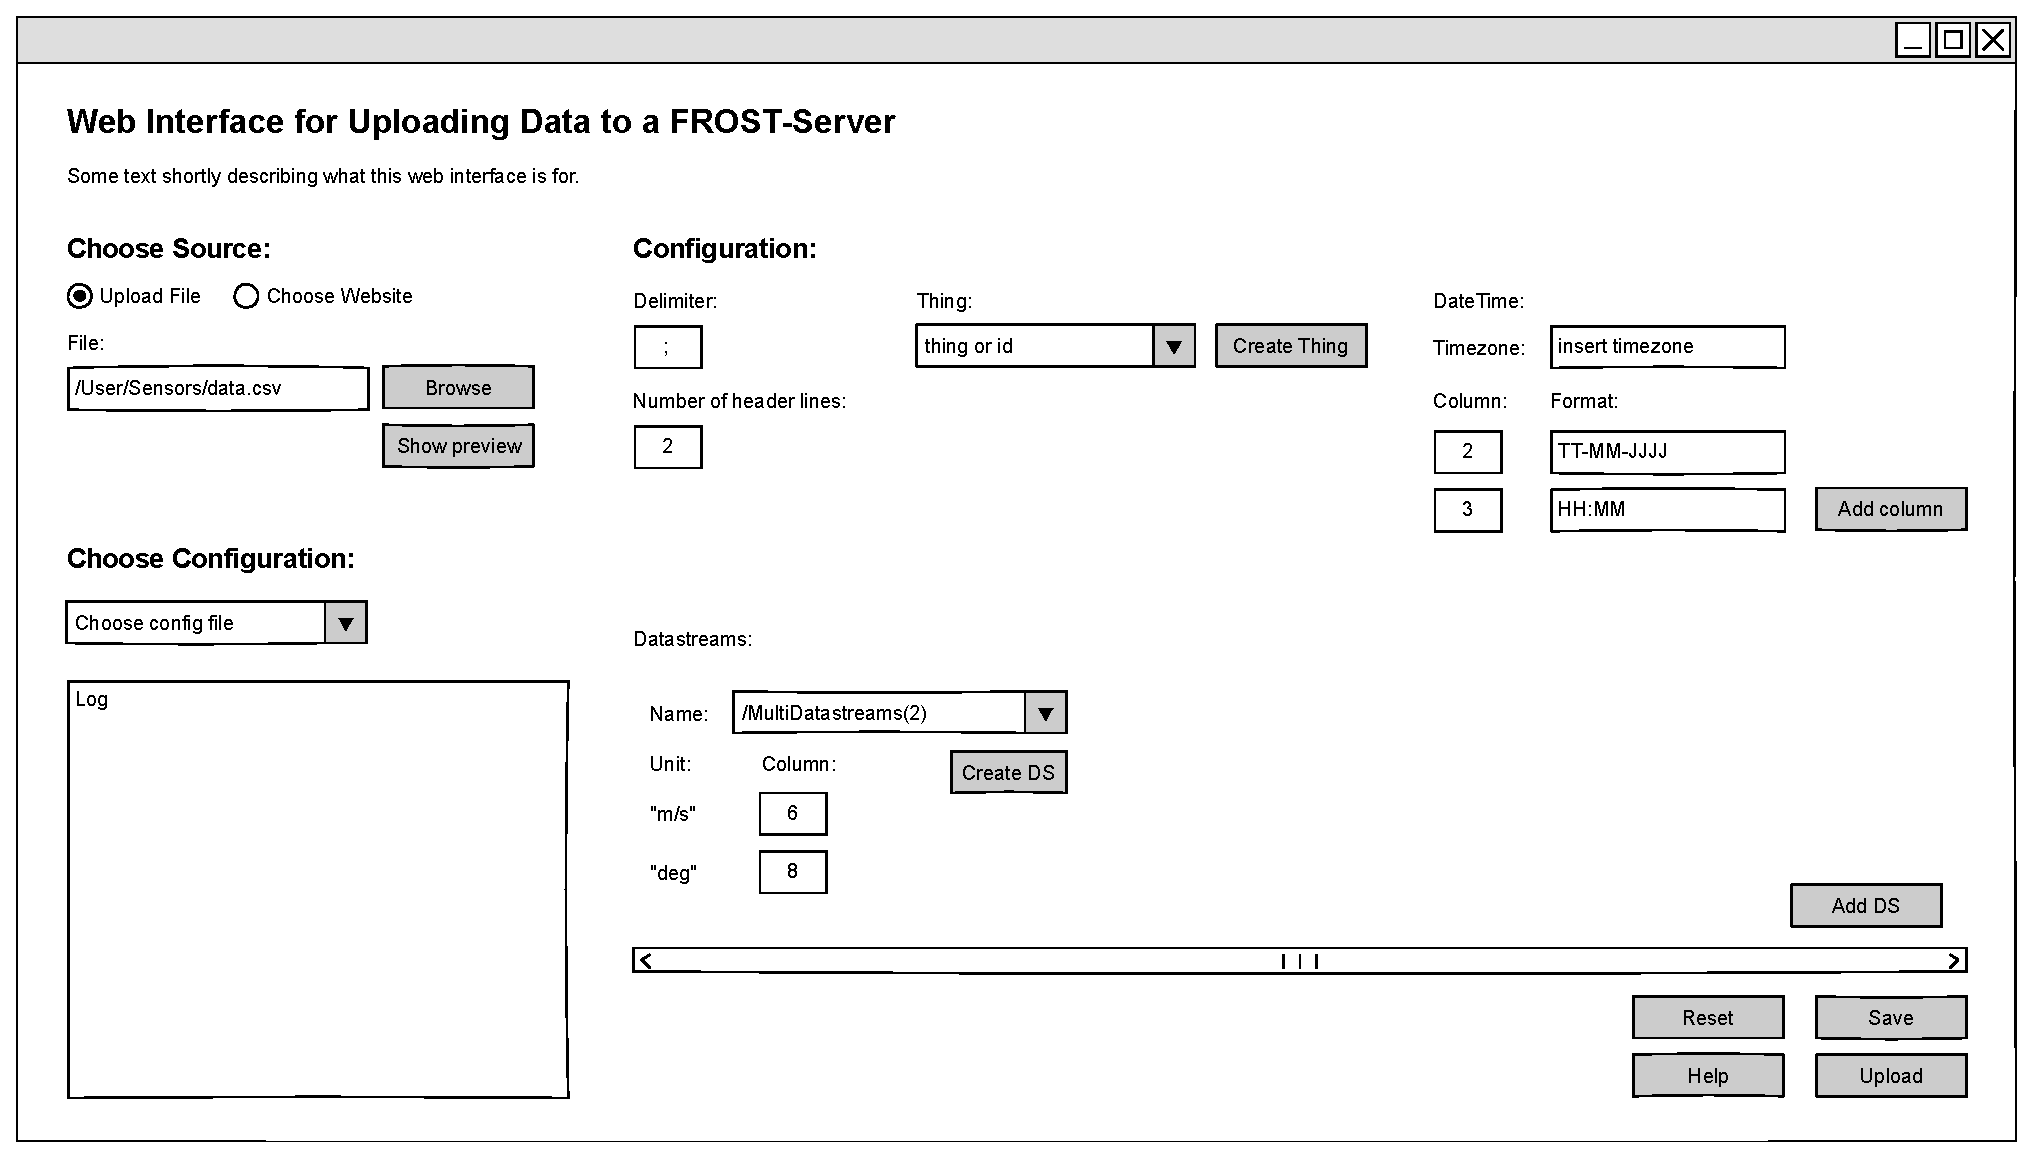
\includegraphics[scale=0.4, angle=90]{images/gui}
\caption{\label{fig:guiMain}Hauptseite der Weboberfläche}
\end{figure}

\begin{figure}[ht]
\centering
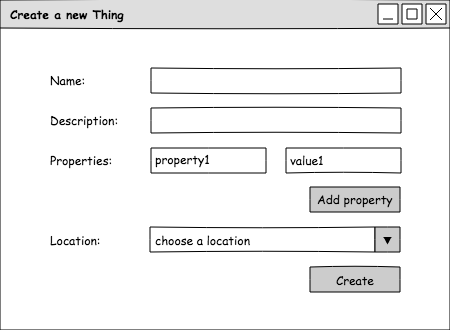
\includegraphics[scale=1]{images/create_thing}
\caption{\label{fig:thing}Dialogfenster zum Erstellen eines Things.}
\end{figure}

\begin{figure}[ht]
\centering
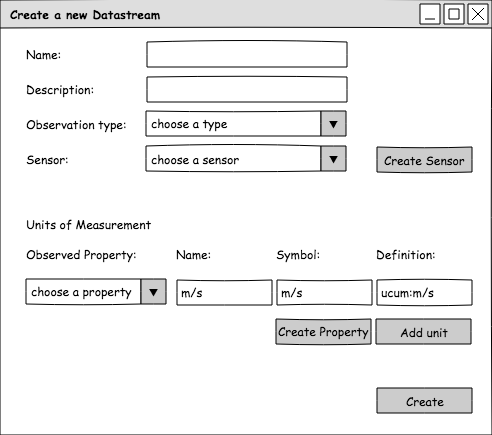
\includegraphics[scale=1]{images/create_datastream}
\caption{\label{fig:ds}Dialogfenster zum Erstellen eines Datastreams.}
\end{figure}

\begin{figure}[ht]
\centering
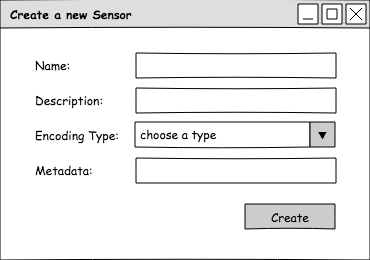
\includegraphics[scale=1]{images/create_sensor}
\caption{\label{fig:sensor}Dialogfenster zum Erstellen eines Sensors.}
\end{figure}

\begin{figure}[ht]
\centering
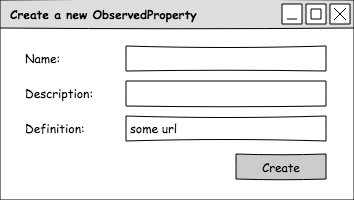
\includegraphics[scale=1]{images/create_observedproperty}
\caption{\label{fig:obsProp}Dialogfenster zum Erstellen eines Things.}
\end{figure}

\subsection{Funktionale Anforderungen}

\begin{itemize}
\item Kurzanleitung auf der Weboberfläche: Auf der Weboberfläche existiert die Möglichkeit, eine Anleitung angezeigt zu bekommen. Diese soll kurz beschreiben, wie der Konfigurator und die Weboberfläche an sich funktionieren.
\item Auswahlmöglichkeit des Zielservers: Auf der Weboberfläche soll ein ereichbarer Frost-Server zum Hinterlegen der Daten einstellbar sein
\item Auswahlmöglichkeit der Datenquelle: Auf der Weboberfläche lässt sich auswählen, ob eine Datei (.csv/.xlsx) hochgeladen, eine entfernte Web-Adresse als Quelle dient oder Daten aus einem schon bestehenden Server importiert werden sollen.
\item Auswahlmöglichkeit einer Konfiguration: Auf der Weboberfläche besteht die Möglichkeit eine Konfigation abzuspeichern und eine abgespeicherte Konfiguration erneut zu laden.
\item Bereitstellen einer Default-Konfiguration
\item Konfiguration zum Laden der Daten auf den Frost-Server: Auf der Weboberfläche lassen sich das Format der hochzuladenden Daten einstellen. Dazu wird die Auswahl bzw. das Neuanlegen eines Things und zugehörigen Datastreams ermöglicht. Außerdem lässt sich das Datumsformat in der Daten in der Quelldatei festlegen.
\item Hochladen der Daten auf den Frost-Server
\item Formatieren der Daten: Vor dem Abspeichern auf dem Frost-Server werden die Daten formatiert, sodass sie dem OGC SensorThings API Standard enstprechen.
\item Anlegen einer Log-Datei: Während der Nutzung der Weboberfläche wird eine Log-Datei erstellt, die sämtliche Aktionen des Nutzers sowie Weboberfäche/Server-Interaktionen aufzeichnet, um Fehlererkennung und -verfolgung zu erleichtern.
\item Sprachauswahl
\item Auswahlmöglichkeit komplexer Operationen auf Daten: Auf der Weboberfläche lassen sich komplexere Datentransformationen auswählen. Diese sollen das Abspeichern von Datenaggregationen wie Summe, MIn, Max und Durchschnitt des Datensatzes ermöglichen
\item Duplikaterkennung: Bevor Daten auf den Frost-Server hochgeladen werden, wird überprüft, ob diese schon existieren, um redundante Daten zu vermeiden.
\item Fehlermeldungen: Kommt es bei der Verarbeitung der Daten zu Problemen, ermöglichen aussagekräftige Fehlermeldungen eine effiziente Korrektur.
\item Rückgabe nicht verarbeiteter Daten: Können Teile des Datensatzes nicht verarbeitet werden, wird eine csv-Datei mit allen fehlerhaften Daten erstellt und an den Nutzer zurückgegeben.
\end{itemize}

\newpage

\begin{itemize}
%TODO GUI-Design von Thing-/Datastream-Erstellung
	%TODO Units Of Measurement bei Erstellung von Datastreams
%TODO Funk. Anf. Thing-/Datastream-Erstellung
\item Hilfe-Button: Durch Klick wird die README-Datei im Browser aufgerufen
\item Speichern-Button: Bei Klick auf diesen Button wird der Upload der Daten in die Datastreams/MultiDatastreams auf den FROST-Server angestoßen

\item Radio-Boxen "Datei auswählen"/"Web-Adresse angeben": Durch Auswahl einer der Boxen wird entweder die Textbox zur Eingabe des Weblinks der entfernten Datei freigeschaltet oder der "Durchsuchen"-Button zur Auswahl einer lokalen
\item Durchsuchen: Durch Klick auf den "Durchsuchen"-Button öffnet sich der Datei-auswählen-Systemdialog, bei dem man die Datei auswählen kann. Im Systemdialog wird das Dateiformat auf entweder CSV oder XLS/XLSX begrenzt. Nachdem die Datei im Systemdialog ausgewählt wurde, wird sie auf die Größe überprüft und bei erfolgreicher Prüfung hochgeladen.

\item Textbox "Ziel": Hier wird die Adresse des FROST-Servers angegeben
\item Button "Auswählen": Durch Klick auf diesen Button wird die im Textfeld "Ziel" angegebene Adresse überprüft und durch einen Haken und im Log bestätigt. (Es sollte überprüft werden ob eine Verbindung hergestellt werden kann,ob eventuell Zugriffsrechte benötigt werden und ob die Zieladresse überhaupt zu einem FROST-Server führt) 

\item Konfiguration durchsuchen/laden: Durch Klick auf "Durchsuchen" öffnet sich der Datei-auswählen-Systemdialog in dem man die CFG-Konfigurationsdatei auswählen kann. Die Konfiguration wird geprüft und anschließend geladen.
\item Konfiguration speichern: Durch Klick auf den Button "Speichern" wird der Download der aktuellen Konfiguration als CFG-Datei gestartet
\item Reset-Button: Bei Klick auf den Reset-Button wird die gesamte Konfiguration (Datums-/Zeitformat, Datastreams, Ziel) zurückgesetzt

\item Thing- / id-Dropdown-Menü: Ein existierendes Thing kann anhand des Namens oder der ID aus einer Liste ausgewählt werden
\item Button "Neu": Existiert ein Thing noch nicht so kann es durch den Button "neu" erstellt werden. Es öffnet sich eine Dialogbox, die es ermöglicht ein neues Thing zu erstellen

\item Textfelder "Spalte": Hier kann durch Angabe der Spaltennummern eingestellt werden in welchen Spalten das Datum/die Uhrzeit zu finden ist
\item Textfelder "Format": Hier wird per RegEx-String eingestellt, in welchem Format das Datum in den Spalten vorliegt
\item Button "+": Hier können mehr Spalten, die das Datum beinhalten, ausgewählt werden

\item "Name"-Dropdown-Menü: Hier kann der (Multi-)Datastream über seinen Namen oder seiner ID aus einer Liste ausgewählt werden
\item Spalten-Textfelder: Hier kann zu der vorangehenden Einheit die Spalte, die den Wert enthält, angegeben werden
\item Button "Neu": Durch Klick auf den Button öffnet sich ein Dialogfenster, welches das Erstellen eines neuen (Multi-)Datastreams ermöglicht
\item Button "+": Durch klick auf den Button "+" wird eine neue Box von Feldern erstellt, in der man Spalten auf Werte eines Datastreams abbilden kann

\item Textfeld "Name": Hier kann der Name des neuen Things eingegeben werden. Dieser kann frei gewählt werden, darf aber nicht leer sein.
\item Textfeld "Description": Hier kann eine Beschreibung des Thing in einem oder mehreren Worten eingegeben werden. Die Beschreibung kann auch ausgelassen werden.
\item Textfeld "Property" (bsph. belegt durch property1): Hier kann der Name einer Property (siehe SensorThings API -> Things -> Properties) eingetragen werden
\item Textfeld "Value" (bsph. belegt durch value1): Hier kann zur Property der Wert eingetragen werden. Werte "true"/"false" werden automatisch zu Boolean umgewandelt, Zahlenwerte zu Integer/Float und Textwerte zu Strings
\item Button "Add Property": Hier wird ein neues Textfeld-Paar Property/Value zum Interface hinzugefügt, damit mehrere Properties eingetrage werden können
\item Dropdown-Menü "Location": Hier ann der derzeitge ort des Things aus einer Liste aus Orten ausgewählt
\end{itemize}


%TODO Nummerierung der Wunschkriterien in Fließtext
\subsection{Produktdaten}
Die gesicherten Daten der Software sind minimal, konkret heißt das es wird nur ein Log-File gesichert. Die Konfiguration wird dem Nutzer per CFG-Datei zum Download bereitgestellt und nicht Serverseitig gespeichert.\\
Sollte das Kriterium [Wunsch: Automatischer Download] mit aufgenommen werden, so muss die Adresse der entfernten Datei und des zu nutzenden FROST-Servers auf dem Server gespeichert werden.
\begin{itemize}
\item Log-Datei
\item Abspeichern der Konfigurationen
\item Speichern der Domain des FROST-Servers auf dem Server
\item Speichern der Domain der entfernten CSV-Adresse auf dem Server
\end{itemize}

\subsection{Produktleistungen}
Die Software soll sämtliche Aktionen der Nutzer in einem Log-File speichern. Die Eingaben sollen möglichst direkt verarbeitet und die Reaktionszeit möglichst gering sein. Bei langsamen Operationen soll der Nutzer Feedback über eine Fortschrittsleiste und über das Log-Fenster bekommen. \\
Die Daten müssen korrekt an den FROST-Server übermittelt werden, dazu gehört auch Robustheit der Anwendung gegenüber falschen Angaben. Bei falschen Angaben oder sonstigen Fehlern soll der Nutzer mittels einer Fehlermeldung benachrichtigt werden.
\begin{itemize}
\item Logging
\item Statusmeldungen an den Nutzer
\item Schnelle Reaktionszeit auf Benutzer-Eingaben
\item korrekte Übertragung der Daten
\item Robustheit gegenüber falschen Formatangeben (Fehlermeldungen)
\end{itemize}

\subsection{Nichtfunktionale Anforderungen}
Die Software ist Open-Source und benötigt einen erreichbaren FROST-Server. Sie basiert auf der SensorThings-API, welche wie der FROST-Server ebenfalls Open-Source ist.
Das Programm wird in Java geschrieben und hängt dementsprechend von einer Java-Umgebung ab.
Um Sicherheit zu gewährleisten sollte das Programm robust gegenüber schädlichen Anfragen sein, vor allem zu große oder zu viele Anfragen sollten dementsprechend abgelehnt werden um eine Überlastung des Servers zu vermeiden.
Außerdem sollten die daten HTTPS-/SSL-Verschlüsselt werden um Abfangen der daten zu verhindern.

(einzuhaltende Gesetze, Normen, Urheber- und Markenrechte,
Sicherheitsanforderungen, Plattformabhängigkeiten)
\begin{itemize}
\item Genutzt wird der FROST-Server und die SensorThings API (beides Open-Source)
\item Die Software ist Open-Source (GPLv3)
\item Die Software ist abhängig von der Java-Plattform
\item Robustheit gegenüber zu großen bzw. zu vielen Anfragen 		
\item HTTPS-/SSL-Verschlüsselung								
\end{itemize}


\subsection{Qualitätsanforderungen}
Das Programm sollte über lange Zeiträume auch ohne Unterbrechungen zuverlässig ausgeführt werden können, solange die Produktumgebung dies zulässt.
Die Benutzbarkeit hat höchste Priorität, auch Nutzer ohne oder wenig technischem Vorwissen sollten in der Lage sein die Software zu bedienen.
Außerdem soll es möglichst einfach sein die Software schnell und unkompliziert zu ändern oder zu erweitern.
Eine einfache Portierung ist gegeben, da die Software auf Java basiert und damit Platformunabhängig ist. Es wird lediglich eine Produktumgebung vorausgesetzt die die Betriebsbedingungen erfüllt.

(In diesem Kapitel wird den Qualitätsmerkmalen Funktionalität, Zuverlässigkeit, Benutzbarkeit, Effizienz, Änderbarkeit und Übertragbarkeit je eine Qualitätsstufe aus sehr gut, gut, normal und nicht relevant zugeordnet.)
\begin{itemize}
\item Die Software sollte zuverlässig auch über längere Zeiträume ohne Unterbrechung laufen sofern es die Produktumgebung zulässt
\item Die Benutzbarkeit hat höchste Priorität, es soll auch Nutzern mit wenig Computerkentnissen möglich sein die Software zu bedienen
\item Es soll einfach möglich sein, Änderungen und Erweiterungen an der Software vorzunehmen
\item Die Software ist einfach zu übertragen, da sie auf der plattformunabhängigen Programmiersprache Java basiert, es wird nur eine Produktumgebung vorausgesetzt, die lediglich die Betreibsbedingungen erfüllt
\end{itemize}

\subsection{Anwendungsszenarien}
Ideen für Anwendungsszenarien:
%TODO Anwendungsfalldiagramm
\begin{itemize}
\item Nutzer ohne technische Kenntnisse des Frost Server Aufbaus besitzt einen Frost Server und einen Sensor, der schon auf dem Frost Server abgespeichert ist. Außerdem hat er eine csv-Datei mit Daten vom Sensor, der einen schon bestehenden Datensatz des Sensors auf dem Server erweitern soll. Er navigiert in seinem Browser zur Web-oberfläche und stellt seine Datei als Quelle und den Frost Server als Ziel ein. Dann wählt er eine Favoritenkonfiguration aus, die zu seinem Sensor passt und lädt seine Daten durch Klick des "Upload"-Buttons hoch. Die Daten werden formatiert und auf dem Server abgrspeichert.
\item das gleiche mit einem erfahrenen Nutzer, der ein neues Thing, einen Sensor und zugehörigen Datastream erstellt
\item Szenario zum Abspeichern einer Konfiguration
\end{itemize}


\subsection{Testfälle}
\test{Default Case zum }{}

\test{Anzeigen der Weboberfläche}{}
\ \\
\teststep{Der Nutzer hat einen Browser geöffnet.}{Der Nutzer navigiert auf die Webseite.}{Die Webseite wird angezeigt wie in \cref{fig:guiMain} dargestellt.}
\ \\
\test{Datei als Quelle wählen}{}
\ \\
\teststep{Dem Nutzer wird die Webseite angezeigt.}{Der Nutzer wählt die Radio-Box "{Upload File}".}{Es wird ein Textfeld und ein "Browse"-Knopf angezeigt, um die hochzuladende Datei festzulegen.}
\ \\
\teststep{}{Der Nutzer drückt den "{Browse}"{-Knopf}.}{Es öffnet sich ein Dateimanager zum Auswählen der Datei.}
\ \\
\teststep{}{Der Nutzer wählt seine Datei aus.}{Der Dateipfad erscheint im Textfeld.}
\ \\
\test{Entfernte Webseite als Quelle wählen}{}
\ \\
\teststep{Dem Nutzer wird die Webseite angezeigt.}{Der Nutzer wählt die Radio-Box "{Choose Website}".}{Es wird ein Textfeld angezeigt, um die URL der entfernten Webseite festzulegen.}
\ \\
\teststep{}{Der Nutzer gibt eine URL ein.}{Die URL wird auf Gültigkeit überprüft und die zu ladende Datei auf dem Server der Weboberfläche zwischengespeichert.}
\ \\
\test{Zielserver wählen}{}
\ \\
\teststep{Dem Nutzer wird die Webseite angezeigt. Insbesondere existiert ein Textfeld zur Eingabe des Zielservers.}{Der Nutzer gibt einen FROST-Server als Ziel in das Textfeld ein und drückt den "{Submit}"{-Knopf}.}{Der Server wird auf Gültigkeit überprüft und bei Korrektheit erscheint ein Konfigurator zum Einstellen des Formats der Daten in der Quelldatei. Im Konfigurator ist der Default-Case voreingestellt.}
\ \\
\test{Konfiguration zurücksetzen}{}
\ \\
\teststep{Der Nutzer befindet sich auf der Webseite und es wird der Konfigurator angezeigt.}{Der Nutzer drückt den "{Reset}"{-Knopf}.}{Alle eingestellten Konfigurationen werden auf den Default-Case zurückgesetzt.}
\ \\
\test{Hilfe anfordern}{}
\ \\
\teststep{Der Nutzer befindet sich auf der Webseite.}{Der Nutzer drückt den "{Hilfe}"{-Knopf}.}{Es wird eine Anleitung für den Gebrauch der Weboberfläche angezeigt.}
\ \\
\test{Konfiguration abspeichern}{}
\ \\
\teststep{Der Nutzer hat eine Konfiguration erstellt.}{Der Nutzer drückt den "{Save}"{-Knopf}.}{Es wird eine cfg-Datei der Konfiguration erstellt und der Download der Datei wird angestoßen.}
\ \\
\test{Konfiguration laden}{}
\ \\
\teststep{Der Nutzer befindet sich auf der Webseite und hat eine gültige Quelldatei und einen gültigen Zielserver angegeben. Es wird ein Konfigurator angezeigt.}{Der Nutzer drückt den "{Browse}"{-Knopf}.}{Es öffnet sich ein Dateimanager.}
\ \\
\teststep{}{Der Nutzer wählt eine cfg-Datei.}{Die Datei wird auf Korrektheit überprüft und im Erfolgsfall ist der Konfigurator entsprechend der Datei eingestellt.}

\ \\
\test{Sensor erstellen}{}
\ \\
\teststep{Der Nutzer erstellt gerade einen Datastream (sieht den Dialog \ref{fig:ds}) und der zugehörige Sensor existiert noch nicht.}{Der Nutzer drückt den "{Create Sensor}"{-Knopf}.}{Es öffnet sich das Dialogfenster zum Erstellen eines Sensors (vgl \ref{fig:sensor}).}
\ \\
\teststep{}{Der Nutzer füllt alle Textfelder aus und drückt den "{Create}"{-Knopf}.}{Die Daten werden überprüft und ein neuer Sensor wird angelegt. Das Dialogfenster wird geschlossen.}

\ \\
\test{ObervedProperty erstellen}{}
\ \\
\teststep{Der Nutzer erstellt gerade einen Datastream (sieht den Dialog \ref{fig:ds}) und eine ObservedProperty für einen Datensatz existiert noch nicht.}{Der Nutzer drückt den "{Create Property}"{-Knopf}.}{Es öffnet sich das Dialogfenster zum Erstellen einer ObservedProperty (vgl \ref{fig:obsProp}).}
\ \\
\teststep{}{Der Nutzer füllt alle Textfelder aus und drückt den "{Create}"{-Knopf}.}{Die Daten werden überprüft und ein neue ObservedProperty wird angelegt. Das Dialogfenster wird geschlossen.}
\ \\

\test{Einen Datensatz zu einem Datastream hinzufügen}{}
\ \\
\teststep{Der Nutzer erstellt gerade einen Datastream (sieht den Dialog \ref{fig:ds}).}{Der Nutzer drückt den "{Add unit}"{-Knopf}.}{Es wird eine neue leere Zeile in der Tabelle für die zum Datastream gehörigen Units of Measurement angelegt.}														  			   
		
												  			   
\test{Einstellen nichts neu}{}
\teststep{Der Nutzer hat Quelle und Ziel eingegeben und bestätigt}{Der Nutzer füllt die Datums-/Uhrzeits-Spalte aus}{Die Software überprüft die Korrektheit der Spalten (Wurde eine Spalte angegeben, die nicht existiert?)}
\teststep{Die Spalten wurden korrekt angegeben}{Der Benutzer gibt via RegEx das Format des Datums/der Uhrzeit in dem dazugehörigen Textfeld an}{Die Korrektheit des RegEx wird anhand der Werte der Tabellendatei auf Fehler geprüft}
\teststep{Das Datum / die Uhrzeit wurde korrekt ausgefüllt}{Der Nutzer wählt das Thing aus dem Dropdown-Menü, welches alle Things enthält, aus}{Das Datastream-Dropdown-Menü wird mit den zum gewählten Thing gehörenden Data-/MultiData-Streams aktualisiert}
\teststep{Thing wurde ausgewählt}{Der Anwender wählt den Datastream aus dem Datastream-Dropdown-Menü aus}{Das System lädt die zum Datastream/MultiDataStream gehörenden Messeinheiten neben die Textfelder zum eintragen}
\teststep{Messdaten geladen}{Der Nutzer trägt die Spalten mit den Messwerten neben die Messeinheiten ein}{Die Korrektheit der Eintragung wird wieder durch die Software geprüft}
\teststep{Alle Textfelder ausgefüllt}{der User klickt auf den Button "{Upload}"}{Die Daten in den angegebenen Spalten werden eingelesen, konvertiert und auf den FROST-Server übertragen}

\test{Neue Datums-/Zeit-Spalte erstellen}{}
\teststep{Der Nutzer hat die Datei geladen und den Server angegeben, es wird keine CFG-Datei genutzt (Ende von Test 1-fach)}{Der Benutzer drückt den "+"-Button, um eine neue Datums-/Zeit-Spalte anzulegen}{Die Software erstellt zwei neue Textfelder mit "Spalte" und "Format" im Interface, sodass sich die Datums- und Zeitnagabe über mehrere Spalten erstrecken kann}

\test{Datastream hinzufügen}{}
\teststep{Ein Thing wurde ausgewählt, die Datastreams wurden in das Dropdown-Menü geladen}{Der Nutzer klickt auf den "{Add DS}"{-Button}}{Das Webinterface wird aktualisiert und rechts vom letzten Datastream wird ein neues Dropdown-Menü für einen neuen Datastream und neue Textfelder hinzugefügt}

\test{Neues Thing erstellen}{}
\teststep{Die Datei und die FROST-Server-Domain wurden angegeben/hochgeladen}{Der Nutzer klickt auf den "{Create Thing}"{-Button}}{es öffnet sich der "{Create New Thing}"{-Dialog}}
\teststep{Das Dialogfenster ist offen, Name und Beschreibung des Things wurden in die Textfelder eingetragen, die Location wurde aus dem Dropdown-Menü ausgewählt}{Der Nutzer klickt auf "{Create}"}{Das Thing wird auf dem FROST-Server erstellt und in dem Hauptinterface dem Dropdown-Menü hinzugefügt}

\test{Properties hinzufügen}{}
\teststep{Der "{Create New Thing}"{-Dialog} ist offen}{Der Nutzer klickt einmal oder mehrfach auf den "{Add Property}"{-Button}}{es werden ein oder mehrere Textfeld-Paare im Interface erstellt in denen der Nutzer die Eigenschaft (Property) und den Wert (Value) des Things einstellen kann}
	
\test{Neuen (Multi)DataStream erstellen}{}
\teststep{Die Datei und FROST-Server wurden angegeben und ein Thing ausgewählt}{Der User klickt auf den "{Create DS}"{-Button}}{Es öffnet sich der "{Create New DataStream}"{-Dialog} indem der User einen neuen DataStream oder MultiDataStream formulieren und erstellen kann}
\teststep{Der User sieht das Dialogfenster zum erstellen eines DataStreams}{der User trägt Name und Beschreibung in die Textfelder ein, wählt Observation Type und Sensor aus den Dropdown-Menüs aus, trägt eine oder mehrere Units Of Measurement ein und klickt abschließend auf "{Create}"}{Die Software unterscheidet zwischen DataStream und MultiDataStream und legt den entsprechenden Stream mit den angegeben Daten im FROST-Server an}


\subsection{Zeitplanung}
Beispielhafte Terminplanung: \\
\begin{itemize}
	\item 07.05. - 27.05.: Pflichtenheft
	\item 28.05. - 24.06.: Entwurfsphase
	\item 25.06. - 22.07.: Implementierung
	\item 23.07. - 12.08.: Beispiel-Urlaubstermin (2 Wochen)
	\item 13.08. - 02.09.: Qualitätssicherung
	\item 03.09. - 09.09.: Terminfenster interne Abnahme
	\item 10.09. - 17.09.: Terminfenster Abschlusspräsentation
\end{itemize}


\subsection{Glossar}
\begin{itemize}
\item FROST \\
	Der \textbf{FR}auenhofer \textbf{O}penSource \textbf{S}ensor\textbf{T}hings-Server ist die erste komplette quelloffene Implementierung der OGC SensorThings API
\item OGC \\
	Das \textbf{O}pen \textbf{G}eospatial \textbf{C}onsortium ist eine gemeinnützige Organisation, die sich zum Ziel gesetzt hat, die Entwicklung von raumbezogener Informationsverarbeitung (insbesondere Geodaten) auf Basis allgemeingültiger Standards festzulegen.
\item SensorThings API \\
	Allgemeiner einheitlicher Standard um Verbindung zwischen Sensoren, deren Ort und Umgebung und den von ihnen erzeugten Daten herzustellen.
\item CSV-/XLSX-Dateien \\
	CSV (Comma Seperated Value, .csv) und Excel (.xlsx) sind gängige Dateiformate zum Speichern von Daten (hier speziell: Sensor-Daten) in Tabellenform.
\item CFG-Datei \\
	Konfigurationsdateien(kurz: CFG-Dateien) sind Textdateien, die speziell zur Speicherung bestimmter Einstellungen (Konfigurationen) dienen.
\item Thing \\
	Ein Thing (deutsch: Ding) ist nach Definition der SensorThings API ein Objekt der physischen oder virtuellen Welt. Es benötigt einen Namen und eine Beschreibung. Es können sich ein oder mehrere Datastreams auf ein Thing beziehen.
\item Datastream \\
	Ein Datastream ist eine fortlaufende Sammlung von Messungen (Observations) des selben Sensors.
\item Integer \\
	Mit Integer wird in der Informatik ein Datentyp bezeichnet, der ganzzahlige Werte speichert.
\item NULL \\
	Als Nullwert (kurz NULL) bezeichnet man in der Informatik einen Zustand, der das Fehlen eines Wertes anzeigen soll.
\item Magic Numbers \\
	Deutsch: Magische Zahl. Ein im Quellcode eines Programms auftauchender Zahlenwert, dessen Bedeutung sich nicht unmittelbar erkennen lässt.
\item Log-Datei \\
	Eine Log-Datei, auch Protokoll-Datei, enthält das automatisch geführte Protokoll aller oder bestimmter Aktionen von Prozessen auf einem Computersystem.
\item Docker \\
	Docker ist eine Software zur Isolierung von Anwendungen. Docker vereinfacht die Bereitstellung von Anwendungen, weil sich sog. Container, die alle nötigen Pakete enthalten, leicht als Dateien transportieren und installieren lassen.
\item GUI \\
	Ein Grafische Benutzeroberfläche (engl. \textbf{G}raphical \textbf{U}ser \textbf{I}nterface) hat die Aufgabe, eine Anwendungssoftware auf einem Rechner mittels grafischer Symbole und Steuerelemente für den Benutzer bedienbar zu machen.
\item (Java) JRE \\
	Mit der Java-Laufzeitumgebung (\textbf{J}ava \textbf{R}untime \textbf{E}nvironment) werden Programme (Java-Anwendungen) weitgehend unabhängig vom darunter liegenden Betriebssystem ausgeführt.
\item JavaScript \\
	JavaScript ist eine Programmiersprache, die hauptsächlich auf Webbrowsern Anwendung findet.
\item headless Server \\
	Als headless (kopflos) bezeichnet man Computer, meist Serversysteme, die über keinen Bildschirm oder sonstige grafische Ausgabe verfügen.
	Diese Systeme haben als Steuerungsmöglichkeit in vielen Fällen eine Netzwerkverbindung.
\item README \\
	Als README (deutsch: Liesmich) wird eine Datei bezeichnet, die üblicherweise mit Software mitgeliefert wird und diverse, oft wichtige Informationen über die Software enthält.
\item Regex \\
	\textbf{Reg}ular \textbf{Ex}pressions (Regex, regulärer Ausdrucke) dienen der Beschreibung von Zeichenketten mit ähnlichem Format.
	Sie können als Filterkriterien in der Textsuche verwendet werden, indem der Text mit dem Muster des regulären Ausdrucks verglichen wird.
\item HTTPS/SSL \\
	\textbf{H}yper\textbf{T}ext \textbf{T}ransfer \textbf{P}rotocol \textbf{S}ecure (HTTPS) ist ein sicheres Hypertext-Übertragungsprotokoll, das SSL benutzt.
	SSL steht für \textbf{S}ecure \textbf{S}ockets \textbf{L}ayer und ist die Standardtechnologie für die Absicherung von Internetverbindungen und den Schutz sensibler Daten, die zwischen zwei Systemen übertragen werden.
\item GPLv3 \\
	GPLv3 ist die aktuelle Version von GPL. Diese \textbf{G}eneral \textbf{P}ublic \textbf{L}icense (allgemeine Veröffentlichungsgenehmigung) ist die am weitesten verbreitete Softwarelizenz,
	die einem gewährt, die Software auszuführen, zu studieren, zu ändern und zu verbreiten.
\end{itemize}


\end{document}